\documentclass[a4paper]{article}

\usepackage{times}
\usepackage{tikz}
\usepackage[margin=0cm]{geometry}
\usepackage{graphicx}
\usepackage{anyfontsize}
\usepackage{fancyhdr}
\usepackage{indentfirst}
\usepackage{amsmath}
\usepackage[spanish]{babel}
\usepackage[utf8]{inputenc}
\usepackage{titlesec}
\usepackage{enumitem}
\usepackage{caption}

\author{}
\date{}
\title{}

\begin{document}
\thispagestyle{empty}

\begin{tikzpicture}[remember picture, overlay]
    \pgftransformshift{\pgfpoint{0cm}{0cm}}
    \draw [line width=2pt](1cm,-1cm) -- (1cm,-27.7cm) -- (14cm, -27.7cm) -- (14cm, -1cm) -- (1cm, -1cm);
    \draw[line width=2pt] (15cm, -27.7cm) -- (19cm,-27.7cm) -- (19cm, -1cm) -- (15cm, -1cm) --  (15cm, -27.7cm);
    \node [line width=2pt] at (17cm, -3.5cm) {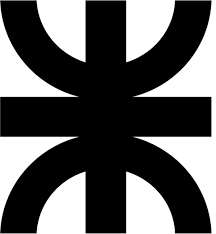
\includegraphics[width=3cm]{../utn.png}};
		\node [line width=2pt] at (7.5cm, -7.5cm) {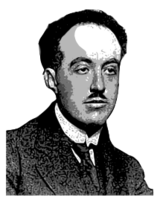
\includegraphics[width=6cm]{../broglie.png}};
    \node at (17cm, -7cm) {\scalebox{5}{\textbf{U}}};
    \node at (17cm, -9cm) {\scalebox{5}{\textbf{T}}};
    \node at (17cm, -11cm) {\scalebox{5}{\textbf{N}}};
    \node at (17cm, -14cm) {\scalebox{5}{\textbf{F}}};
    \node at (17cm, -16cm) {\scalebox{5}{\textbf{R}}};
    \node at (17cm, -18cm) {\scalebox{5}{\textbf{C}}};
    \node at (7.5cm, -12cm) {\scalebox{2.5}{\textbf{Longitud de onda}}};
    \node at (7.5cm, -13cm) {\scalebox{2.5} {\textbf{de \textit{DeBroglie}}}};

    \node at (7.5cm, -23cm) {
        \begin{minipage}[c]{12cm}
            \begin{itemize}
                \raggedright
                \vspace{1.5cm}
                \item \fontsize{12}{12}\selectfont \textbf{Autores:} \vspace {1mm} \fontsize{11}{12}\selectfont \\
                    \hspace{2mm} Valentino Rao - Leg. 402308 \\
                    \hspace{2mm} Ignacio Ismael Perea - Leg. 406265 \\
                    \hspace{2mm} Manuel Leon Parfait - Leg. 406599 \\ 
                    \hspace{2mm} Gonzalo Filsinger - Leg. 400460 \\ 
                    \hspace{2mm} Agustín Coronel - Leg. 402010 \\
                    \hspace{2mm} Marcos Raúl Gatica - Leg. 402006 \\

                \item \fontsize{12}{12}\selectfont \textbf{Curso:} 2R1. \\
                \item \fontsize{12}{12}\selectfont \textbf{Asignatura:} Física electrónica. \\
                \item \fontsize{12}{12}\selectfont \textbf{Institución:} Universidad Tecnológica Nacional - Facultad Regional de Córdoba \\

            \end{itemize}
        \end{minipage}};

\end{tikzpicture}

\renewcommand{\normalsize}{\fontsize{12}{18}\selectfont}
\newgeometry{margin=1cm}
\fancyhf{}
\renewcommand{\headrulewidth}{0pt}
\renewcommand{\footrulewidth}{0pt}
\fancyfoot[R]{[Rao V. - Parfait M. - Filsinger G. - Perea I. - Coronel A - Gatica M.] [\textbf{pág. \thepage}]}
\setlength{\footskip}{0pt}
\newpage
\thispagestyle{empty}
\text{}

\titleformat{\section} {\fontsize{12}{12}\bfseries}{\thesection.}{0.5em}{\underline}

\newpage
\newpage

\thispagestyle{empty}
\setcounter{page}{0}
\tableofcontents

\newpage
\thispagestyle{fancy}
\twocolumn
\flushbottom
formulas
\section{INTRODUCCIÓN}

    \indent El siguiente informe busca introducir el concepto de \textit{Ondas de DeBroglie} y el analísis de sus características corpusculares y de onda.

    \subsection{El principio de dualidad}
        \indent Con el descubrimiento de las propiedades corpusculares de las ondas en 1905, surge la hipótesis de que las partículas se comportan como tal aunque no exista una base experimental firme que la respalde. Esto último logró aportar \textit{Louis de Broglie en 1924}. \\
        
    \subsection{Las ondas de \textit{DeBroglie}}
        \indent Las ondas de \textit{DeBroglie} son aquellas cuya longitud de onda puede ser descripta por: \\

        \begin{center}
            $\lambda = \frac {h} {p}$ \\
        \end{center}
        
        \indent Siendo: \\
        \begin{itemize} [itemsep = -1.5em, topsep = 0em, leftmargin = 1cm]
            \item $\lambda$ = longitud de onda asociada a la partícula. \\
            \item \textit{h} = constante de Planck. \\
            \item \textit{p} = momento lineal de la partícula. \\
        \end{itemize}

        \indent Esto describe el comportamiento ondulatorio de las partículas según la teoría de la dualidad onda-partícula. 

        \indent La demostración de este descriptor parte de conocer la longitud de onda de un fotón de luz: \\

        \begin{equation}
            p = \frac {hv} {c} \tag*{\textit{Momento del fotón.}}  \\
        \end{equation}

        \begin{equation}
            p = \frac {h} {\lambda} \tag*{\textit{Momento en función de la longitud de onda.}} \\
        \end{equation}

        \begin{equation}
            \lambda = \frac {h} {p} \tag*{\textit{Despeje de la long. de onda.}} \\
        \end{equation}

        \indent Siendo \textit{p} el momento lineal del fotón, podemos decir que equivale a: \\

        \begin{equation}
            p = m v \tag*{}
        \end{equation}

        \indent Donde: \\
        \begin{itemize} [itemsep = -1.5em, topsep = 0em, leftmargin = 1cm]
            \item \textit{p} = momento lineal de la partícula. \\
            \item \textit{m} = masa relativista de la partícula. \\
            \item \textit{v} = velocidad de la partícula. \\
        \end{itemize}

        \indent Sabiendo el momento lineal del fotón, podemos concluir en que las \textit{Ondas de DeBroglie} es:

        \begin{equation}
        \lambda = \frac {h} {mv} \tag*{\textit{\textbf{Ondas de DeBroglie}}} \\
        \end{equation}

        \newpage
        \noindent

        \indent Notése que mientras mayor sea el momento lineal del fotón, menor es la longitud de onda que describe. \\
        \indent La ecuación de ondas de \textit{DeBroglie} han sido demostradas con experimentos relacionados con la drifracción de electrones rápidos en cristales (\textbf{ver título 4 de este informe}). Lo que se busca discutir posteriormente es cómo varían éstas ondas en comparación a las electromagnéticas (variación por los campos eléctricos y magnéticos en el espacio y tiempo) o las mećanicas como el sonido (variación por presión). \\ 

\section{VELOCIDAD DE ONDA DE \textit{DEBROGLIE}}

    \indent Durante la \textbf{INTRODUCCIÓN}, se relacionó el concepto de \textit{Ondas de DeBroglie} con un fotón en movimiento. Se espería que la velocidad de propagación sea igual a la que tiene el cuerpo en movimiento: 

    \begin{align}
    \omega &= v \lambda \tag*{\textit{Siendo $\omega$ la velocidad de la onda.}} 
    \end{align}

    \indent Sabiendo que: 

    \begin{align}
        \lambda &= \frac {h} {mv} \tag*{\textit{Onda DeBroglie}} \\[10pt]
        E &= h v \tag*{\textit{Ecuación cuántica}} \\[10pt]
        v &= \frac {E} {h} \tag*{} \\[10pt]
        E &= mc^2 \tag*{\textit{Equiv. masa-energía}} \\[10pt]
        v &= \frac {mc^2} {h} \tag*{} 
    \end{align}

    \indent Por consiguiente la velocidad de onda viene dada por:

    \begin{align}
        \omega &= v \lambda \tag*{} \\[10pt]
        \omega &= (\frac {m c^2} {h}) (\frac {h} {mv}) \tag*{} \\[10pt]
        \omega &= \frac {c^2} {v} \tag*{}
    \end{align}
       
    \indent Sin embargo, la conclusión de la ecuación anterior es contradictoria a los postulados de Einstein: la velocidad de onda de \textit{DeBroglie} es siempre mayor a c. Por lo que es evidente decir que v (velocidad de movimiento del cuerpo ondulatorio) es distinto a $\omega$ (la velocidade propagación de la onda que describe). \\

\newpage
\noindent
\thispagestyle{fancy}

\section{VELOCIDADES DE FASE Y GRUPO}
    \indent La amplitud de las ondas de De Broglie de un cuerpo en movimiento refleja la probabilidad de que a éste se le encuentre en un punto y en un momento determinados. La representación de la onda de un cuerpo en movimiento corresponde a la de un paquete de ondas, o grupo de ondas, cuyas ondas constitutivas tengan amplitudes de las que dependa la probabilidad de detectar el cuerpo.\\

    \begin{figure}[h!]
        \centering
        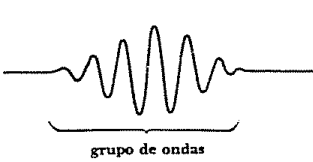
\includegraphics[width = 5.5cm]{../grupoDeOndas.png}
    \end{figure}

    \indent Una manera de describir matemáticamente un grupo de ondas es hacerlo en términos de una superposición de ondas individuales, cada una con longitud de onda diferente, que al interferir entre sí dan por resultado variaciones en las amplitudes que definen la forma del grupo. Si todas las velocidades de onda son iguales, la velocidad con que el grupo de ondas se propaga es idéntica a la común. Sin embargo, si la velocidad de onda varía con la longitud de onda, entonces las ondas individuales no avanzan juntas y el grupo de ondas tiene una velocidad diferente de las ondas que lo componen.\\

    \indent No es difícil calcular la velocidad $\vec{v}$ con que se propaga un grupo de ondas. Supongamos que un grupo de ondas se produce por la combinación de dos ondas de la misma amplitud $A$, pero que difieren en su frecuencia angular y en su constante de propagación $d\omega$  y $dk$, respectivamente. Podemos representar las ondas originales por las fórmulas:

    \begin{align}
        y_1 &= A \cos(\omega t - kx) \tag*{} \\[10pt]
        y_2 &= A \cos[(\omega + d\omega) t - (k + dk)x] \tag*{}
    \end{align}

    \indent El desplazamiento resultante $y$ en un tiempo $t$ y en una posición $x$ es la suma de $y_1$ y $y_2$. Con ayuda de la identidades: \\

    \begin{align}
        \cos(\alpha)+\cos(\beta ) &= 2 \cos(\frac{\alpha+\beta}{2})\cos{(\frac{\alpha-\beta}{2})} \tag*{}
    \end{align}

    \indent Y de la relación

    \begin{align}
        \cos(-\theta)=\cos(\theta) \tag*{}
    \end{align}

    \indent Entonces:

    \begin{align}
        y &= y_1 + y_2 \tag*{} \\[10pt]
        y &= 2A \cos(\frac{(2\omega+ d\omega)t-(2k+dk)k}{2})\cos(\frac{d\omega t-dkx}{2}) \tag*{} 
    \end{align}

    \newpage
    \noindent
    \thispagestyle{fancy}

    \indent Puesto que \( d\omega \) y \( dk \) son pequeños, comparados con \( \omega \) y \( k \): 

    \begin{align}
        2\omega + d\omega &\approx 2\omega \tag*{} \\[10pt]
        2k + dk &\approx 2k \tag*{}
    \end{align}

    \indent Entonces:

    \begin{align}
        y &= 2A \cos(\omega t - kx) \cos(\frac{d\omega t - dkx}{2}) \tag*{} 
    \end{align}

    \indent Esta ecuación representa una onda de frecuencia angular \( \omega \) y constante de propagación \( k \) que tiene superpuesta una modulación de frecuencia angular \( \frac{1}{2}d\omega \) y constante de propagación \( \frac{1}{2}dk \). El sentido de la modulación es producir grupos de ondas sucesivos. \\

    \indent La velocidad de fase \( w \) es:

    \begin{align}
        w &= \frac{d\omega}{dk} \tag*{}
    \end{align}

    \indent y la velocidad de grupo de ondas \( u \)s

    \begin{align}
        u &= \frac{d\omega}{dk} \tag*{}
    \end{align}

    \indent Si la velocidad de fase es la misma para todas las longitudes de onda, son iguales las velocidades de grupo y de fase. La frecuencia angular de De Broglie correspondientes a un cuerpo en movimiento de masa en reposo $m_0$ y velocidad $v$ son:

    \begin{align}
        \omega &= 2\pi v \tag*{} \\[10pt]
        \omega &= \frac{2 \pi mc^2}{h} \tag*{} \\[10pt]
        \omega &= \frac{2 \pi m_0 c^2}{h\sqrt{1-\frac{v^2}{c^2}}} \tag*{} 
    \end{align}

    \indent y su constante de propagación de las ondas:

    \begin{align}
        k &= \frac{2 \pi}{\lambda} \tag*{} \\[10pt]
        k &= \frac{2 \pi}{\frac{h}{p}} \tag*{} \\[10pt]
        k &= \frac{2 \pi mv}{h} \tag*{} \\[10pt]
        k &= \frac{2 \pi m_0 v}{h\sqrt{1-\frac{v^2}{c^2}}} \tag*{}
    \end{align}

    \indent Por lo tanto, $\omega$ y $k$ son funciones de $v$. La velocidad de fase $w$ es:

    \begin{align}
        w &= \frac{\omega}{k} \tag*{} \\[10pt]
        w &= \frac{c^2}{v} \tag*{}
    \end{align}

    \newpage
    \noindent
    \thispagestyle{fancy}

    \indent Y como se puede ver en la última ecuación, la velocidad de fase de las ondas de De Broglie es mayor que la velocidad del objeto y de la luz (como se vió en la sección \textbf{VELOCIDAD DE ONDA DE \textit{DEBROGLIE}}).\\
    \indent La velocidad de grupo $u$ de las ondas de De Broglie del cuerpo es: 

    \begin{align}
        u &= \frac{d\omega}{dk} \tag*{} \\[10pt]
        u &= \frac{d\omega/dv}{dk/dv} \tag*{} 
    \end{align}

    \indent Siendo:

    \begin{align}
        \frac{d\omega}{dv} &= \frac{2 \pi m_0 v}{h(1-v^2/c^2)^{3/2}} \tag*{} \\[10pt]
        y \tag*{}\\[10pt]
        \frac{dk}{dv} &= \frac{2 \pi m_0}{h(1-v^2/c^2)^{3/2}} \tag*{}
    \end{align}

    \indent Por lo tanto, la velocidad de grupo de las ondas de De Broglie es: $u=v$.\\

    \indent En conclusión, la velocidad de fase de las ondas de De Broglie de un cuerpo en movimiento es mayor que la velocidad del cuerpo y de la luz, mientras que la velocidad de grupo es igual a la velocidad del cuerpo.\\

\section{DIFRACCIÓN DE ELECTRONES}

\indent En 1927, Davisson y Germer confirmaron experimentalmente la hipótesis de \textit{DeBroglie} de que los electrones se comportan como ondas demostrando que los mismos se difractan al ser dispersados en cristales en los cuales la separación entre sus átomos tiene una distancia adecuada.\\

    \begin{figure}[h!]
        \centering
        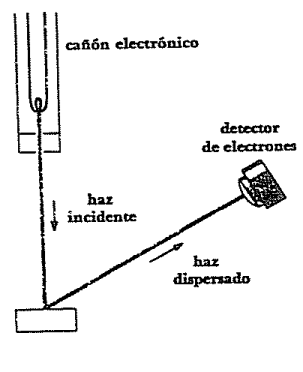
\includegraphics[width = 5.5cm]{../Experimento.png}
    \end{figure}

    \indent En la figura anterior se muestra un esquema del experimento de Davisson y Germer. En el cual se estudiaba la dispersión de electrones en sólidos. La energía de los electrones en el rayo, el ángulo de incidencia sobre el blanco y la posición del detector podían variar. \\

    \newpage
    \noindent
    \thispagestyle{fancy}

    \indent Según física clásica, se predice que los electrones se dispersarán en todas las direcciones sin importar el ángulo de incidencia y la energía de los mismos. Davisson y Germer comprobaron estas prediccones con un bloque de níquel como blanco.\\

    \indent Durante el experimento tuvieron un accidente que dejo entrar aire en el aparato, resultando en la oxidación de la superficie del metal. Para reducir a níquel puro el óxido formado, el blanco se calentó en un horno a altas temperaturas. Luego se volvió a colocar en el aparato y siguieron las mediciones. Los nuevos resultados fueron muy diferentes a los obtenidos antes del accidente, en lugar de una variación continua de la intensidad de los electrones dispersados según el ángulo de incidencia, se observaron máximos y mínimos cuya posición dependía de la energía de los electrones. En la siguiente figura se representan gráficas polares típicas de la intensidad electrónica después del accidente; el método de representación es tal que la intensidad, para cualquier ángulo, es proporcional a la distancia de la curva con ese ángulo, al punto de dispersión.

    \begin{figure}[h!]
        \centering
        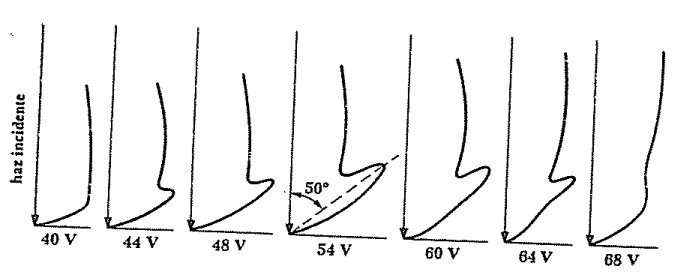
\includegraphics[width = 5.5cm]{../grafica.png}
    \end{figure}

    \indent La hipótesis de De Broglie sugería la interpretación de que las ondas de electrones las difractaba el blanco, en forma similar a como los rayos X son difractados por planos de átomos en un cristal. Esta interpretación se confirmó cuando se aclaró que el calentamiento del bloque producia un solo monocristal a partir de los muchos cristales pequeños que lo componían, quedando todos los átomos dispuestos en una red regular.

    \indent Veamos si se puede verificar que las ondas de De Broglie son la causa del hallazgo de Davisson y Germer. En un cierto experimento, se dirigió un haz de electrones de 54 $eV$ perpendicularmente al blanco de níquel y se observó un máximo en la distribución de electrones en cualquier dirección que formara un ángulo de {50\textdegree} con el haz original. Los ángulos de incidencia y de dispersión relativos a la familia de planos de Bragg (ver dibujo a continuación) serán ambos de {65\textdegree}:

    \begin{figure}[h!]
        \centering
        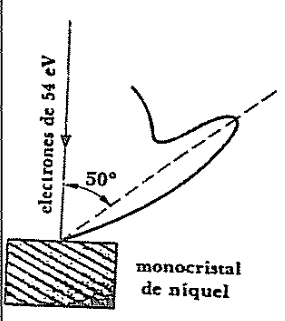
\includegraphics[width = 5.5cm]{../figura3-7.png}
    \end{figure}

    \newpage
    \noindent
    \thispagestyle{fancy}

    \indent La distancia entre planos de esta familia, que se puede medir por difracción de rayos $X$, es 0.91m. La ecuación de Bragg para los máximos en el modelo de difracción es: 


    \begin{align}
        n\lambda &= 2d \sin \theta \tag*{}
    \end{align}

\indent Dando los valores de $n=1$, $d=0.91m$, {$\theta=65$\textdegree}, la longitud de onda de De Broglie $\lambda$ queda:

    \begin{align}
        n\lambda &= 2 \cdot 0.91m  \cdot \sin {65\text{\textdegree}} \tag*{} \\[10pt]
        n\lambda &= 1.65m \tag*{}
    \end{align}

    \indent Con la fórmula de \textit{DeBroglie}: $\lambda=\frac{h}{mv}$. Se puede calcular la longitud de onda de los electrones. La energía cinética del electrón de 54 $eV$ es pequeña comparada con su energía en reposo $m_0c^2$ de $5,1 . 10^5 eV$, asi que no pueden usarse las fórmulas relativistas. Entonces:

    \begin{align}
        K=\frac{mv^2}{2} \tag*{} 
    \end{align}

    \indent El momento del electrón es:

    \begin{align}
        mv &=\sqrt{2mK} \tag*{} \\[10pt]
        mv &=\sqrt{2 \cdot 9.1 \cdot 10^{-31} \, \text{kg} \cdot 54 \, \text{eV} \cdot 1.6 \cdot 10^{-19} \, \text{J/eV}} \tag*{} \\[10pt]
        mv &= 40 \cdot 10^{-24} \, \text{kg} \cdot \text{m/s} \tag*{}
    \end{align}

    \indent La longitud de onda del electrón es:

    \begin{align}
        \lambda &= \frac{h}{mv} \tag*{} \\[10pt]
        \lambda &= \frac{6.63 \cdot 10^{-34} \text{J-s}}{4 \cdot 10^{-24} \text{kg} \cdot \frac {m}{s}} \tag*{} \\[10pt]
        \lambda &= 1.66m \tag*{}
    \end{align}

    \indent Esto concuerda con la longitud de onda observada. El experimento de Davisson y Germer proporciona así una comprobación directa de la hipótesis de De Broglie sobre la naturaleza ondulatoria de los cuerpos en movimiento.\\
    \indent El análisis del experimento de Davisson-Germer no es tan sencillo como en el desarrollo anterior, ya que la energía de un electrón aumenta cuando penetra en un cristal, por lo que la velocidad del electrón es mayor en el interior del cristal, por lo que la longitud de onda de De Broglie es más corta que fuera del cristal. Además, surge una complicación adicional debido a interferencias entre las ondas difractadas por las diferentes familias de planos de Bragg, que restringen la aparición de máximos para ciertas combinaciones de la energía del electrón y del ángulo de incidencia.\\

\indent Como en el caso de las ondas electromagnéticas, los aspectos ondulatorios y corpusculares de los cuerpos en movimiento nunca se pueden observar simultáneamente, de manera que no podemos determinar cuál es la descripción ''correcta''. Por lo que podemos decir que en algunos casos un cuerpo en movimiento muestra propiedades ondulatorias y en otros presenta propiedades corpusculares. 

    \newpage
    \noindent
    \thispagestyle{fancy}

El determinar qué conjunto de propiedades es más evidente depende de la relación entre la longitud de onda de De Broglie y las dimensiones del cuerpo que se considera: la longitud de onda de {$1.66m$} de un electrón de 54 eV es del mismo orden de magnitud que el espaciamiento de la red de un cristal de níquel, pero la longitud de onda de un automóvil que se desplaza a 90 km/h es aproximadamente $1.5 \times 10^{-38}$ m, que es demasiado pequeña para manifestarse.

\section{LA DUALIDAD ONDA-PARTÍCULA}

    \begin{figure}[h!]
        \centering
        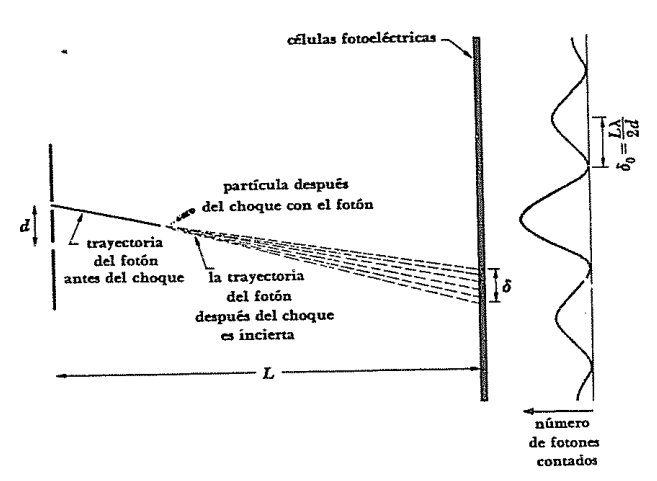
\includegraphics[width = 6.5cm]{../expDualidadOP.png}
    \end{figure}

    \indent Una de las preguntas más difíciles de abordar en física moderna es cómo una partícula puede comportarse tanto como una onda y, en otras circunstancias, como una partícula. A pesar de la existencia de múltiples experimentos que corroboran esta dualidad, la explicación matemática de este fenómeno sigue siendo compleja y no se puede demostrar ambos comportamientos de manera simultánea en un único experimento.

    \indent Consideremos el experimento ilustrado en la figura al inicio de esta sección. Este muestra un dispositivo experimental en el que la luz, al atravesar una doble rendija, se difracta y los fotones son detectados por una serie de células fotoeléctricas dispuestas sobre una superficie de detección. Los fotones, partículas de luz que también exhiben propiedades ondulatorias, producen un patrón de interferencia característico de ondas al ser registrados por los sensores. Si graficamos el número de fotones detectados por cada sensor en función de su posición en la pantalla, obtenemos un patrón de interferencia, similar al de dos trenes de ondas coherentes.\\

    \begin{figure}[h!]
        \centering
        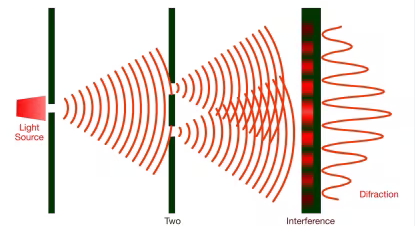
\includegraphics[width = 6.5cm]{../expDOPColor.png}
    \end{figure}

    \indent Este patrón de interferencia persiste incluso cuando la intensidad de la luz es tan baja que, en promedio, solo un fotón pasa a través del aparato en un instante dado. Esto da lugar a cómo puede un único fotón interferir consigo mismo, dicho de otro modo, ¿cómo puede el fotón ''sentir'' la presencia de ambas rendijas cuando, intuitivamente, solo debería pasar por una? \\

    \newpage
    \noindent
    \thispagestyle{fancy}

    \indent Abordar este tema conlleva a realizar una modificación en el experimento: Además de las rendijas, se supondrá hay una nube de partículas entre las rendijas y los sensores. Esta nube permite que, al interactuar un fotón con una partícula en su trayecto, podamos determinar cuál de las dos rendijas ha atravesado. Al detectar el fotón, el choque con una de las partículas de la nube le proporciona un impulso detectable, lo que nos permite inferir la trayectoria seguida por el fotón. Sin embargo, al intentar determinar la trayectoria con precisión, la posición del fotón en el eje $y$ estará sujeta a una incertidumbre $\Delta y$.\\

    \indent Si intentamos reducir esta incertidumbre en la coordenada $y$, la incertidumbre en el momento $p_y$ del fotón aumenta debido al principio de incertidumbre de Heisenberg, de acuerdo con la relación:

    \begin{equation}
        \Delta p_y \geq \frac{h}{\Delta y} > \frac{2h}{d} \tag*{}
    \end{equation}

    \indent Donde $d$ es la distancia entre las dos rendijas. Esta relación establece que cuanto más intentemos localizar al fotón (reducir $\Delta y$), mayor será la incertidumbre en su momento $p_y$. \\

    \indent Debido a este incremento en la incertidumbre del momento en el eje $y$, el fotón sufrirá una desviación adicional en su trayectoria. Este cambio en el momento del fotón, $\Delta p_y$, produce una desviación angular en su camino hacia la pantalla de detección, que se puede expresar como:

    \begin{equation}
        \delta = \frac{\Delta p_y}{p_x} L \tag*{}
    \end{equation}

    \indent Donde: \\

      \begin{itemize} [itemsep = -1.5em, topsep = 0em, leftmargin = 1cm]
        \item $p_x$ = momento en la dirección horizontal. \\
        \item $L$ = distancia entre las rendijas y la pantalla de detección. \\
      \end{itemize}

    \indent Este efecto, derivado de la interacción entre el fotón y las partículas en la nube, introduce suficiente alteración en el sistema para destruir el patrón de interferencia característico de ondas. Este resultado es coherente con la interpretación cuántica: cuando intentamos medir con precisión por cuál rendija pasó el fotón (una propiedad de partícula), el comportamiento ondulatorio desaparece.\\

    \indent El experimento ilustra que la naturaleza cuántica de la luz y otras partículas depende de cómo interactuamos con el sistema. Si medimos el fotón como una partícula, obtenemos información sobre su trayectoria pero perdemos el patrón de interferencia ondulatorio. Por otro lado, si no hacemos ninguna medición que interrumpa el sistema, el fotón parece interferir consigo mismo, comportándose como una onda.


\section{EL MICROSCOPIO ELECTRÓNICO}

    \indent El microscopio electrónico es un ejemplo de las propiedades ondulatorias y corpusculares de los electrones, ya que se puede usar un haz de electrones para formar una imagen de un objeto casi en la misma forma que un rayo de luz. Como la luz se puede desviar haciendo que Los rayos de luz que divergen de un punto en un objeto converjan con una lente convergente o un espejo cóncavo, los electrones que divergen de una región pequeña se pueden hacer converger con campos eléctricos y/o magnéticos.\\

    \indent \textbf{¿Por qué un microscopio electrónico es superior a un microscopio óptico?}\\

    \newpage
    \noindent
    \thispagestyle{fancy}

    \indent Sin importar la calidad de la fabricacion de las lentes para un microscopio óptico, la longitud de onda de la luz visible limita la resolución del microscopio. En cambio, la longitud de onda de los electrones en un microscopio electrónico es mucho más pequeña que la de la luz visible, lo que permite una resolución mucho mayor y que el máximo de aumento posible sea miles de veces mayor.\\

    \subsection{El microscopio electrónico de transmisión}

    \indent En la mayoría de los microscopios electrónicos usan campos magnéticos, y no campos eléctricos, como "lentes" para enfocar el haz. En los microscopios electrónicos de transmisión se usan tres de esas lentes en un arreglo en forma de microscopio compuesto, como se ve en la imagen. Los electrones son emitidos por un cátodo caliente y acelerados por una diferencia de potencial de 10 a 100kV los cuales pasan por una lente condensadora y se conforman en un rayo paralelo. Luego la lente objetivo forma una imagen intermedia de este objeto, y la lente de proyección produce una imagen real final del objeto en una pantalla fluorescente o en una placa fotográfica. Este procedimiento se debe realizar en el vacío. En estos microscopios la muestra a examinar es muy delgada, normalmente de 10 a 100 nm de espesor, por lo que los electrones no se desaceleran en forma apreciable al atravesarlo.\\

    \begin{figure}[h!]
        \centering
        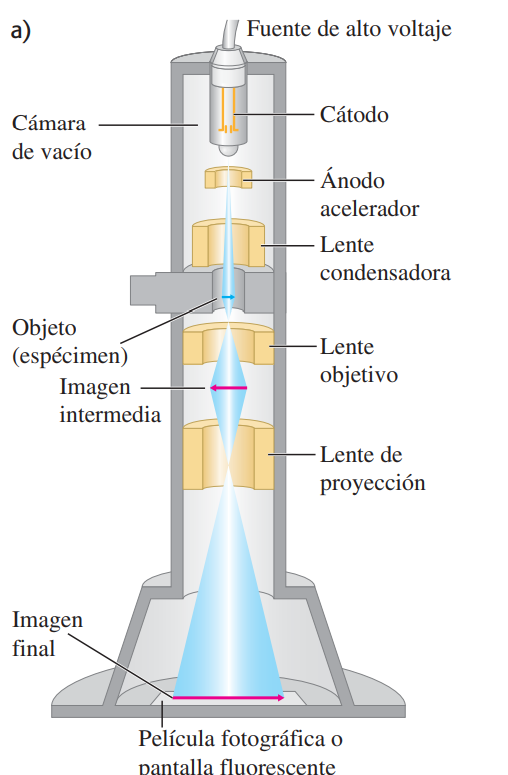
\includegraphics[width = 6.5cm]{../microscopio.png}
    \end{figure}
\subsection{El microscopio electrónico de barrido}

    \indent En el microscopio electrónico de barrido, el haz de electrones se enfoca formando una línea muy fina que barre el espécimen, por lo que los electrones salen despedidos y son reunidos por un ánodo recolector positivo mantenido un potencial de algunos cientos de volts. La corriente en el ánodo recolector se amplifica y usa para modular el haz de electrones en un tubo de rayos catódicos, que es barrido en sincronización con el haz en el microscopio. Así, el tubo de rayos catódicos traza una imagen muy aumentada del espécimen.\\

    \newpage
    \noindent
    \thispagestyle{fancy}

    \indent Algunas ventajas es que el espécimen puede ser grueso, ya que el haz no necesita atravesarlo, y la producción de electrones despedidos depende del ángulo de incidencia del haz, lo que permite que las imagenes sean tridimensionales.\\

    \begin{figure}[h!]
        \centering
        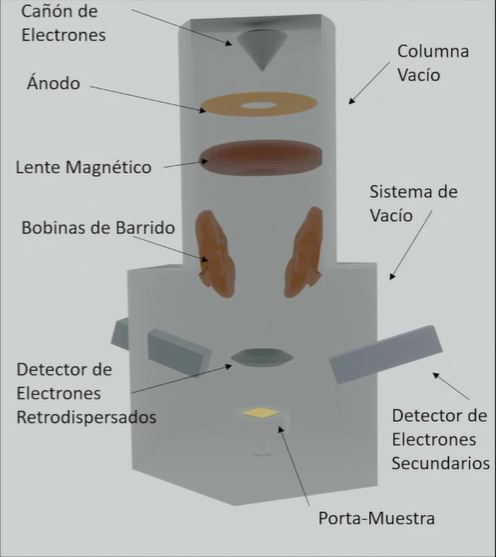
\includegraphics[width = 6.5cm]{../microbarrido.png}
    \end{figure}

\indent \underline{Ejemplos de imágenes:}

    \begin{itemize}
        \item \textbf{Microscopio electrónico de transmisión}
    \end{itemize}

    \begin{figure}[h!]
        \centering
        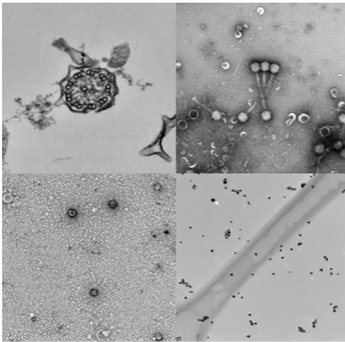
\includegraphics[width = 5cm]{../microtrans.png}
    \end{figure}

    \begin{itemize}
        \item \textbf{Microscopio electrónico de barrido}
    \end{itemize}

    \begin{figure}[h!]
        \centering
        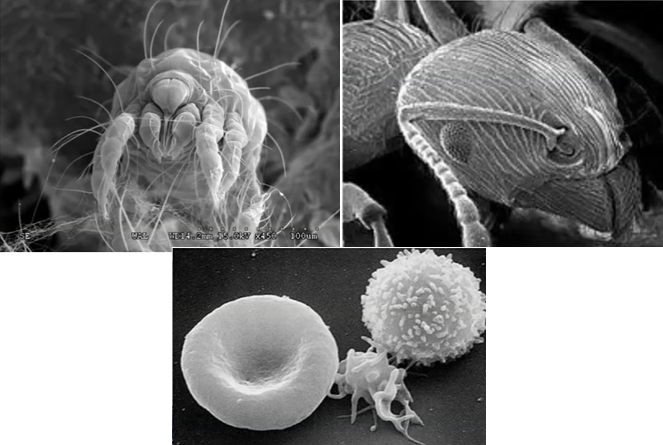
\includegraphics[width = 5cm]{../barrido.png}
    \end{figure}


\end{document}
